\documentclass[a4 paper]{article}
% Set target color model to RGB
\usepackage[inner=2.0cm,outer=2.0cm,top=2.5cm,bottom=2.5cm]{geometry}
\usepackage{setspace}
\usepackage[rgb]{xcolor}
\usepackage{verbatim}
%\usepackage{subcaption}
\usepackage{amsgen,amsmath,amstext,amsbsy,amsopn,tikz,amssymb,tkz-linknodes}
\usepackage{fancyhdr}
\usepackage[colorlinks=true, urlcolor=blue,  linkcolor=blue, citecolor=blue]{hyperref}
\usepackage[colorinlistoftodos]{todonotes}
\usepackage{rotating}
% \usepackage{float}

\usepackage{listings}
\usepackage{color}
\usepackage{graphicx}
\usepackage{floatrow}
\usepackage{subfig}
\usepackage{enumitem}

\usepackage{booktabs}
\newcommand{\ra}[1]{\renewcommand{\arraystretch}{#1}}

\newtheorem{thm}{Theorem}[section]
\newtheorem{prop}[thm]{Proposition}
\newtheorem{lem}[thm]{Lemma}
\newtheorem{cor}[thm]{Corollary}
\newtheorem{defn}[thm]{Definition}
\newtheorem{rem}[thm]{Remark}
\numberwithin{equation}{section}

\newcommand{\homework}[6]{
   \pagestyle{myheadings}
   \thispagestyle{plain}
   \newpage
   \setcounter{page}{1}
   \noindent
   \begin{center}
   \framebox{
      \vbox{\vspace{2mm}
    \hbox to 6.28in { {\bf COL774:~Machine Learning \hfill { #2}} }
       \vspace{6mm}
       \hbox to 6.28in { {\LARGE \hfill #1  \hfill} }
       \vspace{6mm}
       \hbox to 6.28in {\bf {Entry Number: {\rm #4} \hfill Name: {\rm #5} } }
       % \hbox to 6.28in { {\it TA: #4  \hfill #6}}
      \vspace{2mm}}
   }
   \end{center}
   \markboth{#1}{#1}
   \vspace*{4mm}
}

% \newcommand{\problem}[2]{~\\\fbox{\textbf{Problem #1}}\hfill (#2 points)\newline\newline}
% \newcommand{\subproblem}[1]{~\newline\textbf{(#1)}}
% \newcommand{\D}{\mathcal{D}}
% \newcommand{\Hy}{\mathcal{H}}
% \newcommand{\VS}{\textrm{VS}}
% \newcommand{\solution}{~\newline\textbf{\textit{(Solution)}} }

% \newcommand{\bbF}{\mathbb{F}}
% \newcommand{\bbX}{\mathbb{X}}
% \newcommand{\bI}{\mathbf{I}}
% \newcommand{\bX}{\mathbf{X}}
% \newcommand{\bY}{\mathbf{Y}}
% \newcommand{\bepsilon}{\boldsymbol{\epsilon}}
% \newcommand{\balpha}{\boldsymbol{\alpha}}
% \newcommand{\bbeta}{\boldsymbol{\beta}}
% \newcommand{\0}{\mathbf{0}}

\begin{document}
\homework{Assignment 3 Report}{Date: April 7, 2019}{}{\bf 2016CS10363}{\bf Manish Tanwar}{NetId(s)}

\section*{1. Decision Trees:}

\subsection*{Part (a):}
\begin{figure}[ht!]
	\centering %width=90mm
	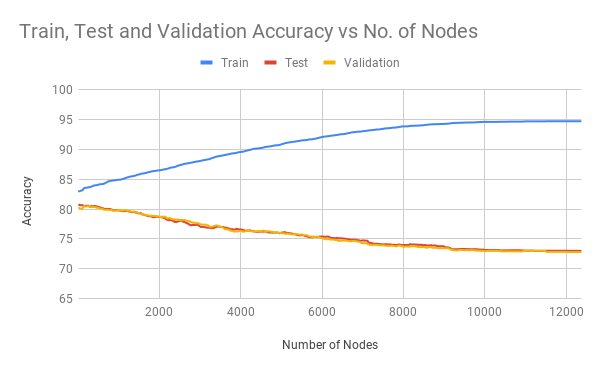
\includegraphics[width=110mm]{./chart/DT_a.png}
	\caption{Accuracy Vs No. of Nodes}
\end{figure}

\subsection*{Part (c):}
\begin{figure}[ht!]
	\centering %width=90mm
	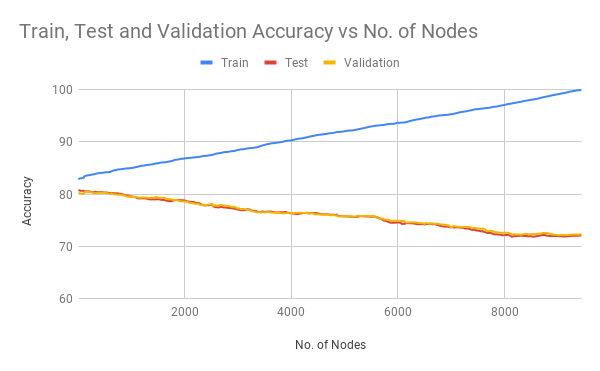
\includegraphics[width=110mm]{./chart/DT_c.png}
	\caption{Accuracy Vs No. of Nodes}
\end{figure}

\textbf{Multisplit Atrributes:}
Following attributes split multiple times along a branch with their maximum number of split along a path from root to node.

\hskip1.0cm\begin{tabular}{ |p{2.7cm}||p{2.5cm} |}
	 \hline
	 % \multicolumn{3}{|c|}{Training Time(in Sec)} \\
	 \hline \textbf{Atrribute} & \textbf{Max No. of Split}\\
	 \hline
	 X1		& 6 \\
	 X5		& 4 \\
	 X12	& 4 \\
	 X13	& 4 \\
	 X14	& 3 \\
	 X15	& 3 \\
	 X16	& 3 \\
	 X17	& 3 \\
	 X18	& 4 \\
	 X19	& 4 \\
	 X20	& 3 \\
	 X21	& 3 \\
	 X22	& 3 \\
	 X23	& 3 \\
	 \hline
\end{tabular}

\subsection*{Part (d):}

\begin{figure}[ht!]
	\centering %width=90mm
	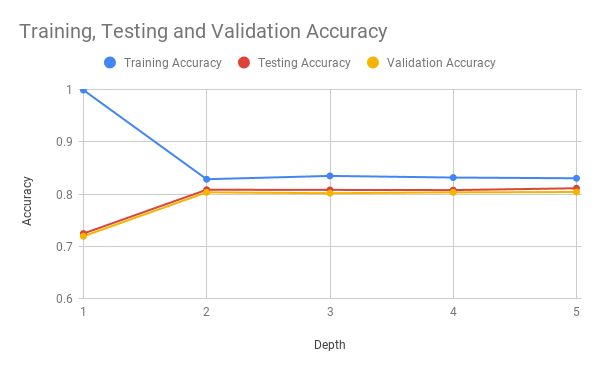
\includegraphics[width=110mm]{./chart/DT_d1.png}
	\caption{Accuracy Vs Depth}
\end{figure}

\begin{figure}[ht!]
	\centering %width=90mm
	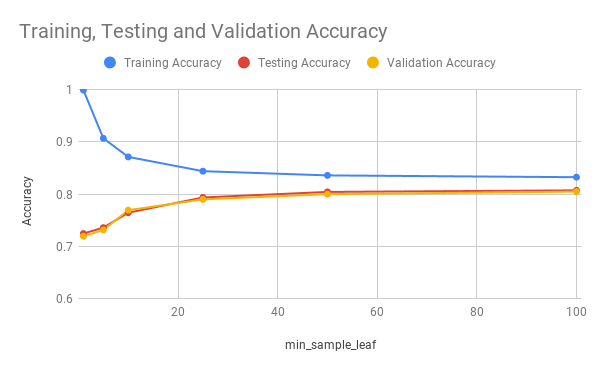
\includegraphics[width=110mm]{./chart/DT_d2.png}
	\caption{Accuracy Vs Min sample leaf}
\end{figure}

\begin{figure}[ht!]
	\centering %width=90mm
	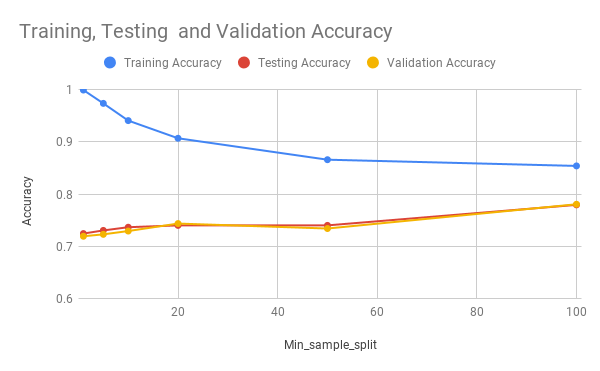
\includegraphics[width=110mm]{./chart/DT_d3.png}
	\caption{Accuracy Vs Min Sample Split}
\end{figure}

\begin{itemize}
\item \textbf{Best Parameters:}
max\_depth = 4, min\_samples\_split = 10, min\_samples\_leaf = 30
\item \textbf{Accuracies Obtained:}  Test Accuracy: 80.85\%, Train Accuracy: 83.20\%, Validation Accuracy: 80.52 \%
\end{itemize}

 
\subsection*{Part (e):}

\begin{itemize}
\item \textbf{Best Parameters:}
max\_depth = 50, min\_samples\_split = 100, min\_samples\_leaf = 50
\item \textbf{Accuracies Obtained:}  Test Accuracy: 80.71\%, Train Accuracy: 83.18\%, Validation Accuracy: 80.45 \%
\end{itemize}

\subsection*{Part (f):}

\begin{itemize}
\item \textbf{Best Parameters:}
n\_estimators=120,  max\_features=2, bootstrap = True
\item \textbf{Accuracies Obtained:}  Test Accuracy: 79.56\%, Train Accuracy: 86.63\%, Validation Accuracy: 79.51 \%	
\end{itemize}

\section*{2. Neural Network:}

\subsection*{Implementation Specifications:}
\begin{itemize}
\item Used Softmax activation function in the output layer.
\item Used cross entropy loss as loss funciton.
\end{itemize}

\subsection*{Part (a):}
One-hot Encoding Dataset Link: \url{https://drive.google.com/drive/folders/1VVqfcNAuw_i5A9KtQhZJur_dFKMND5h1?usp=sharing}


\subsection*{Part (c):}
\begin{itemize}
	\item \textbf{Stopping Criteria:} \\
Stopping criteria is either of these two condition is true:
\begin{enumerate}
\item $\big| Loss(\theta)^{(t+1)} - Loss(\theta)^{(t)} \big| < \epsilon \hspace*{1.65cm} (\text{for a sufficiently small } \epsilon \text{ (took } \epsilon = 10^{-7}))$
\\ where $Loss(\theta)^{t}$ is the loss after $t^{th}$ epoch.
\item Constrainted on number of epochs with 1000.
\end{enumerate}

\item \textbf{Accuracy and Trainig Time:}

\hskip1.0cm\begin{tabular}{ |p{2.7cm}||p{2.5cm}|p{3.3cm}|p{3.3cm}|}
	 \hline
	 % \multicolumn{3}{|c|}{Training Time(in Sec)} \\
	 \hline \textbf{Hiddern Layer Units} & \textbf{Training Time} & \textbf{Training Accuracy} & \textbf{Testing Accuracy}\\
	 \hline
	 5 &  107 sec &  57.24\% & 52.38\% \\
	 10 & 122 sec & 58.7\% &  58.5\% \\
	 15 & 147 sec & 58.8\% &  54\% \\
	 20 & 175 sec & 96.22\% & 93.93\% \\
	 25 & 185 sec & 97.72\% & 95.17\% \\
	 \hline
\end{tabular}


% \begin{figure}[H]
% 	\centering %width=90mm
% 	\includegraphics[width=80mm]{chart/chart1.png}
% 	\caption{Training time vs Number of Hidden Layer Units\label{MIMD}}
% \end{figure}

% \begin{figure}[H]
% 	\centering %width=90mm
% 	\includegraphics[width=80mm]{chart/acc.png}
% 	\caption{Training Accuracy and Testing Accuracy vs Number of Hidden Layer Units}
% \end{figure}

\begin{figure}[H]
\centering
	\begin{floatrow}
	\hspace*{-0.9in}
	  \ffigbox[\FBwidth]{\caption{\small{Training time vs No. of Hidden Layer Units}}}{%
	  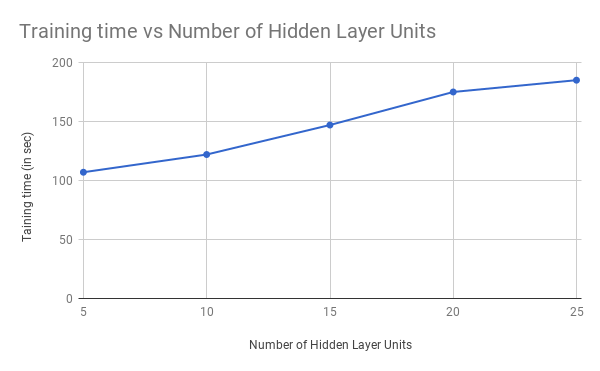
\includegraphics[width=100mm]{chart/c_time.png}
	  }
	  \ffigbox[\FBwidth]{\caption{\small{Training \& Testing Accuracy vs No. of Hidden Layer Units}}}{%
		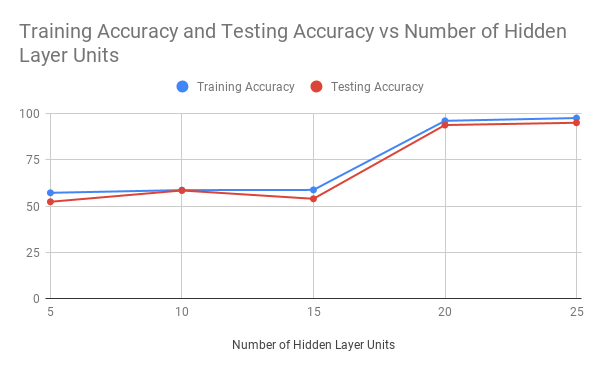
\includegraphics[width=100mm]{chart/c_acc.png}
	  }
\end{floatrow}
\end{figure}


\item \textbf{Confusion Matrices:}

% \begin{figure}[H]
% \centering
% 	\begin{floatrow}
% 	\hspace*{-0.9in}
% 	  \ffigbox[\FBwidth]{\caption{\small{Training time vs No. of Hidden Layer Units}}}{%
% 	  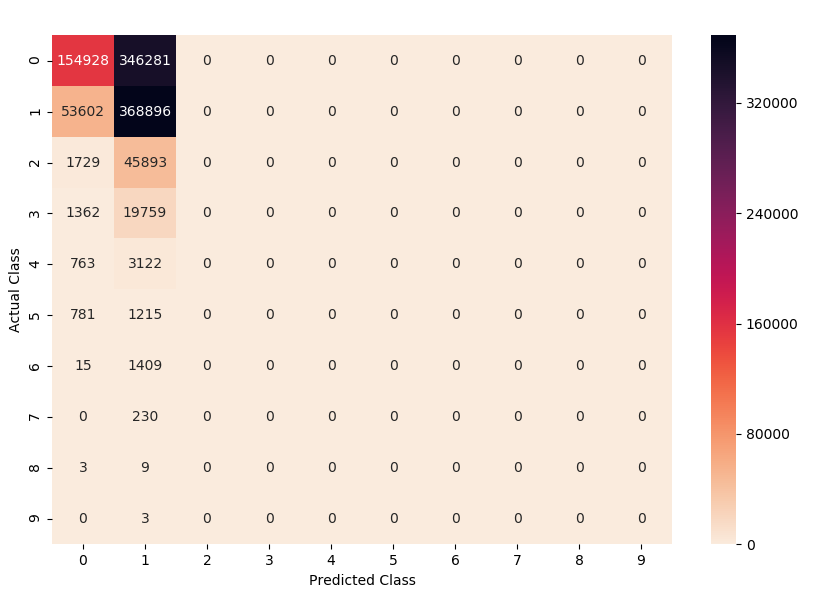
\includegraphics[width=100mm]{chart/c_5.png}
% 	  }
% 	  \ffigbox[\FBwidth]{\caption{\small{Training \& Testing Accuracy vs No. of Hidden Layer Units}}}{%
% 		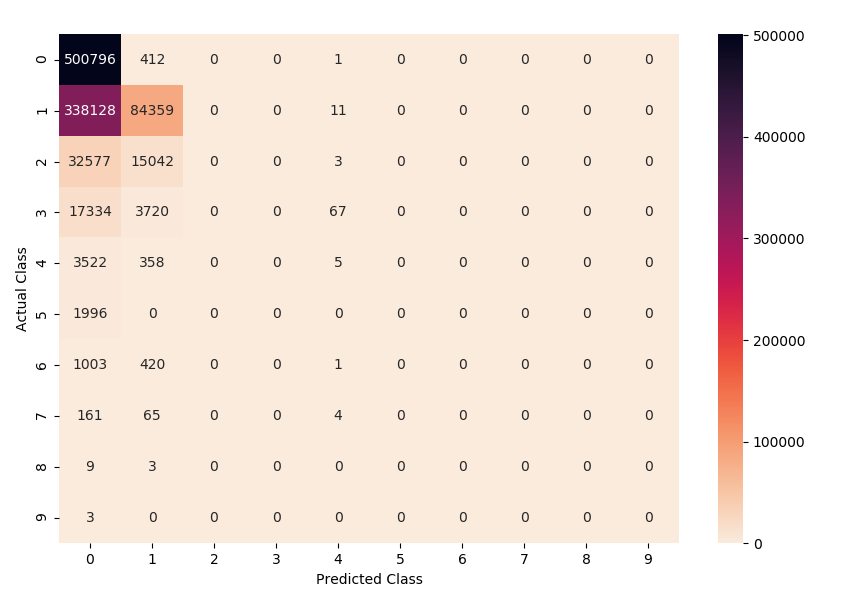
\includegraphics[width=100mm]{chart/c_10.png}
% 	  }

% 	  \ffigbox[\FBwidth]{\caption{\small{Training \& Testing Accuracy vs No. of Hidden Layer Units}}}{%
% 		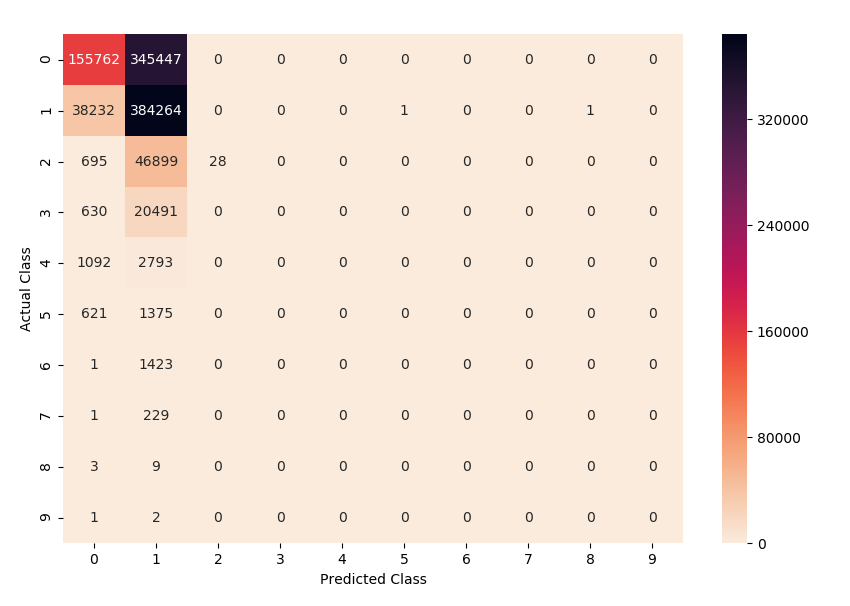
\includegraphics[width=100mm]{chart/c_15.png}
% 	  }
% \end{floatrow}
% \end{figure}

\begin{figure}[H]
    \centering
    \subfloat[]{{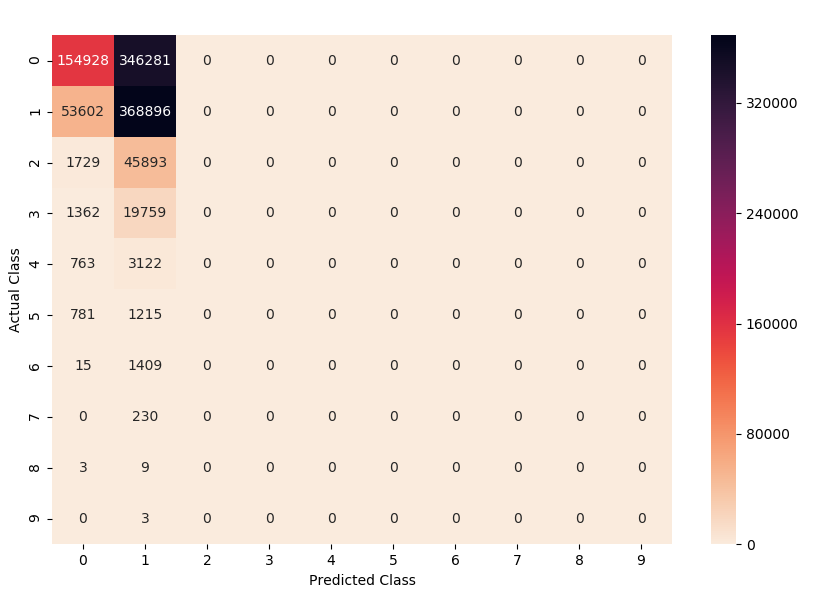
\includegraphics[width=7cm]{chart/c_5.png}} }%
    \subfloat[]{{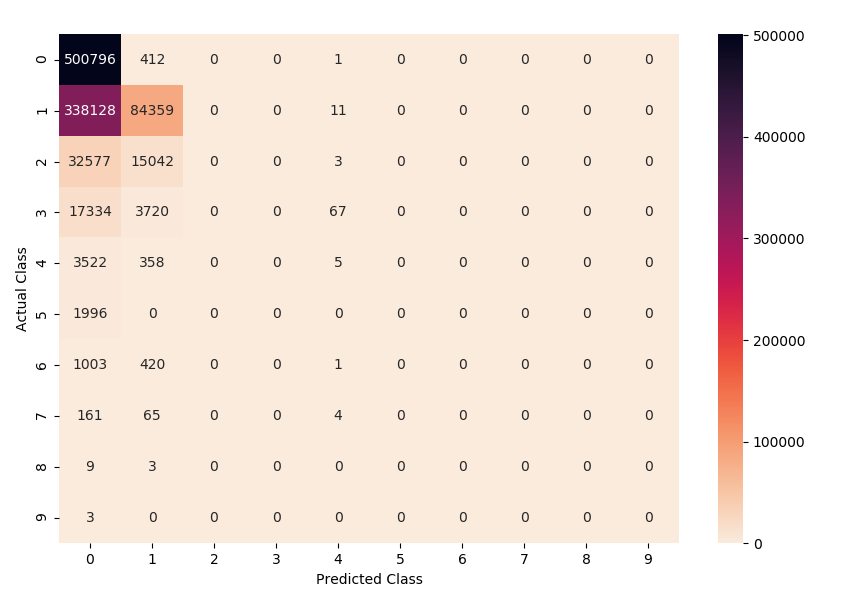
\includegraphics[width=7cm]{chart/c_10.png} }}%
    \qquad
  	\hspace*{-1.5cm}
    \subfloat[]{{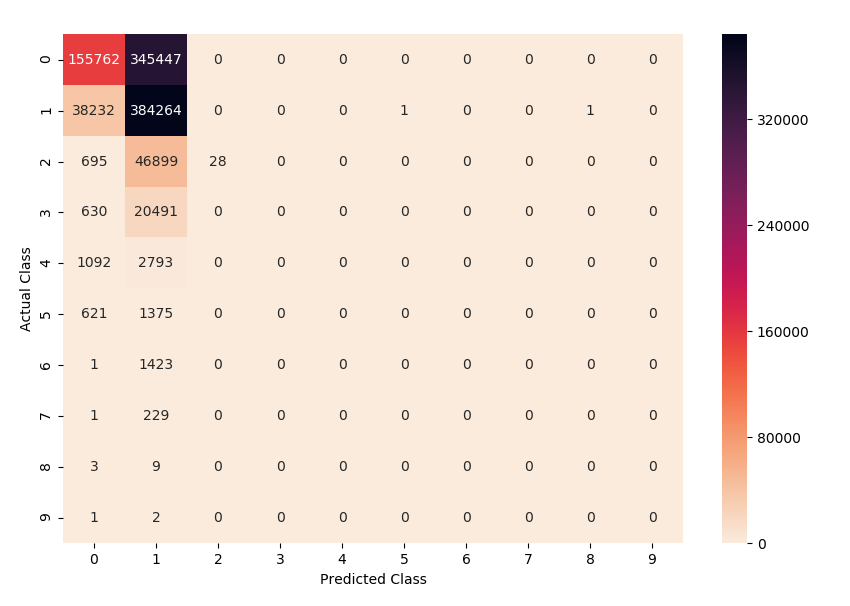
\includegraphics[width=7cm]{chart/c_15.png} }}%
    \subfloat[]{{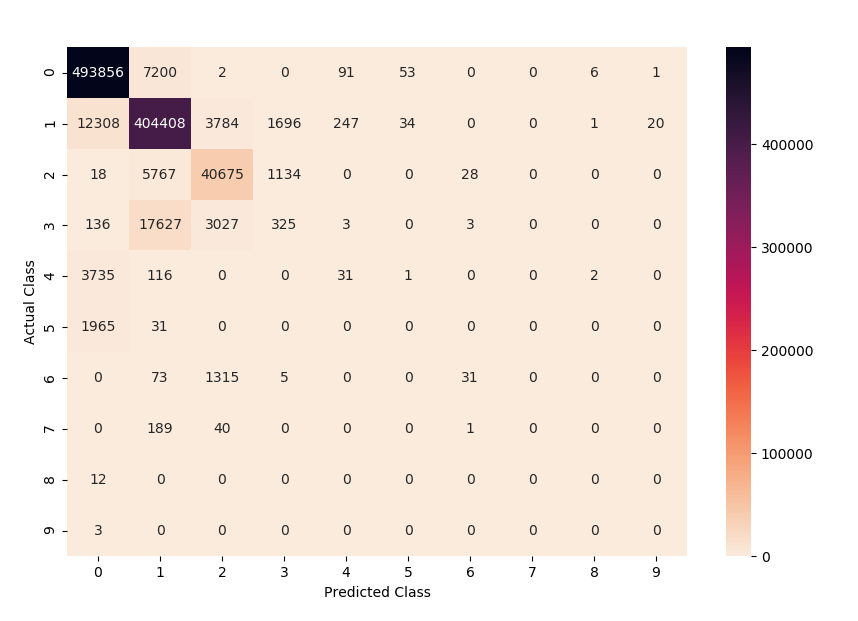
\includegraphics[width=7cm]{chart/c_20.png} }}%
    \subfloat[]{{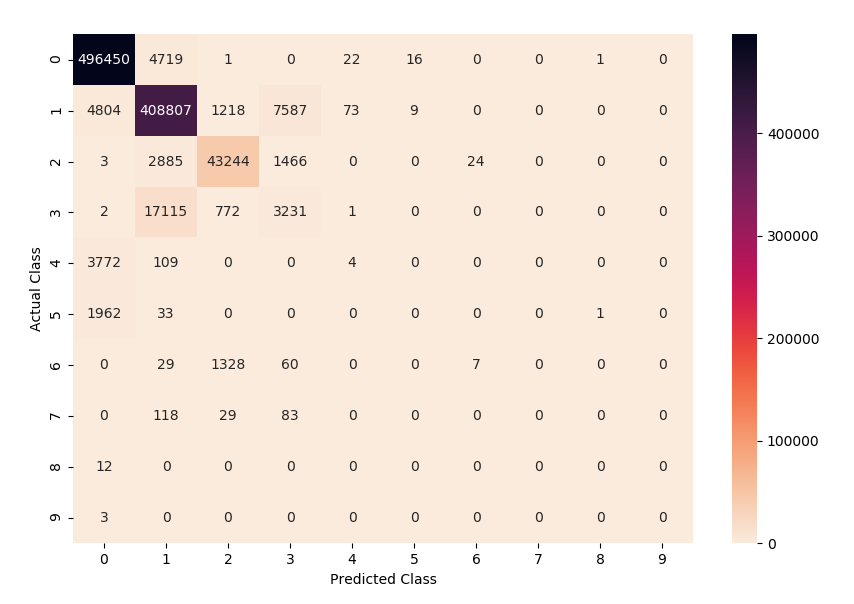
\includegraphics[width=7cm]{chart/c_25.png} }}%
    \caption{Confusion Matrices for hidden layers units = [5,10,15,20,25]}%
    \label{fig:example}%
\end{figure}

\end{itemize}
% ----------------------------------

\subsection*{Part (d): Double Layer:}
\begin{itemize}
\item \textbf{Accuracy and Trainig Time:}

\hskip1.0cm\begin{tabular}{ |p{2.7cm}||p{2.5cm}|p{3.3cm}|p{3.3cm}|}
	 \hline
	 % \multicolumn{3}{|c|}{Training Time(in Sec)} \\
	 \hline \textbf{Hiddern Layer Units(for both layers)} & \textbf{Training Time} & \textbf{Training Accuracy} & \textbf{Testing Accuracy}\\
	 \hline
	 5 &  158 sec & 57.14\% &  55.70\% \\
	 10 & 194 sec & 79.69\% &  78.56\% \\
	 15 & 239 sec & 90.62\% &  89.38\% \\
	 20 & 294 sec & 98.37\% &  96.87\% \\
	 25 & 397 sec & 99.26\% &  96.30\% \\
	 \hline
\end{tabular}

\begin{figure}[H]
\centering
	\begin{floatrow}
	\hspace*{-0.9in}
	  \ffigbox[\FBwidth]{\caption{\small{Training time vs No. of Hidden Layer Units}}}{%
	  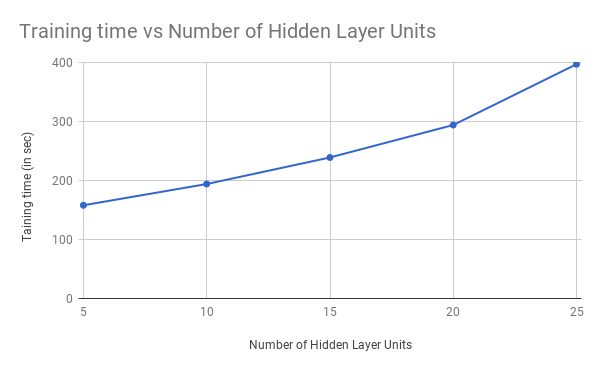
\includegraphics[width=100mm]{chart/d_time.png}
	  }
	  \ffigbox[\FBwidth]{\caption{\small{Training \& Testing Accuracy vs No. of Hidden Layer Units}}}{%
		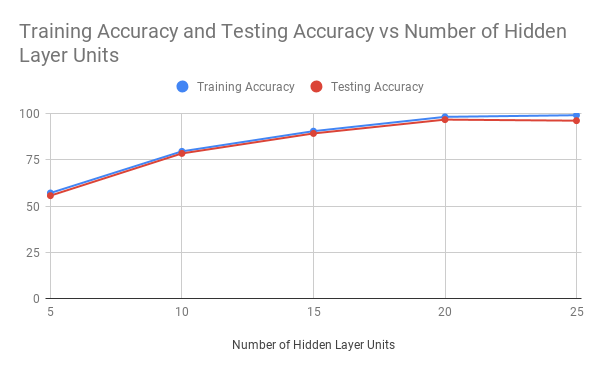
\includegraphics[width=100mm]{chart/d_acc.png}
	  }
\end{floatrow}
\end{figure}


\item \textbf{Confusion Matrices:}
\begin{figure}[H]
    \centering
    \subfloat[]{{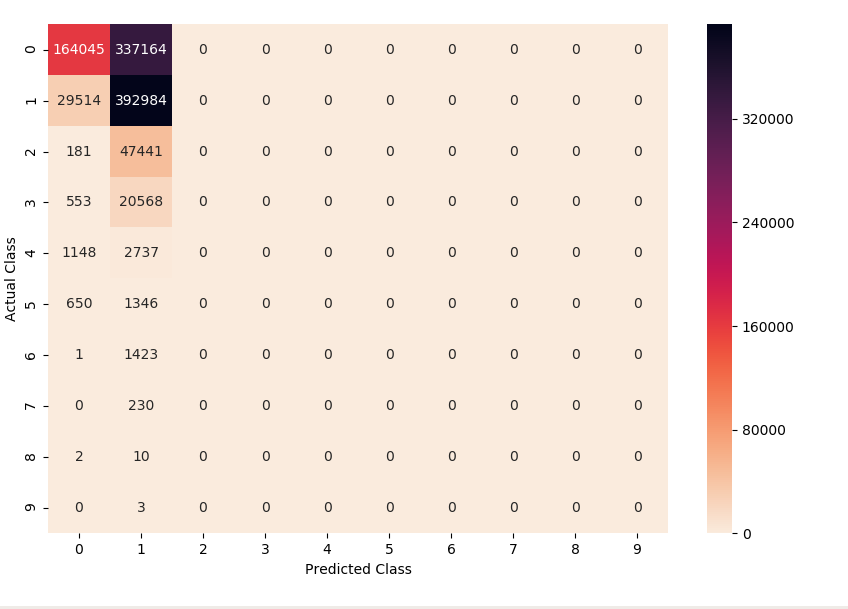
\includegraphics[width=7cm]{chart/d_5.png}} }%
    \subfloat[]{{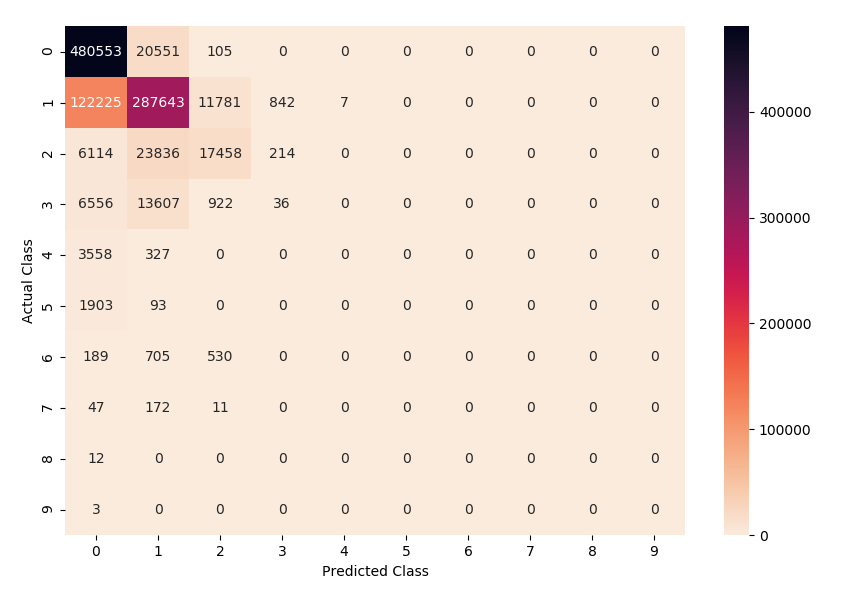
\includegraphics[width=7cm]{chart/d_10.png} }}%
    \qquad
  	\hspace*{-1.5cm}
    \subfloat[]{{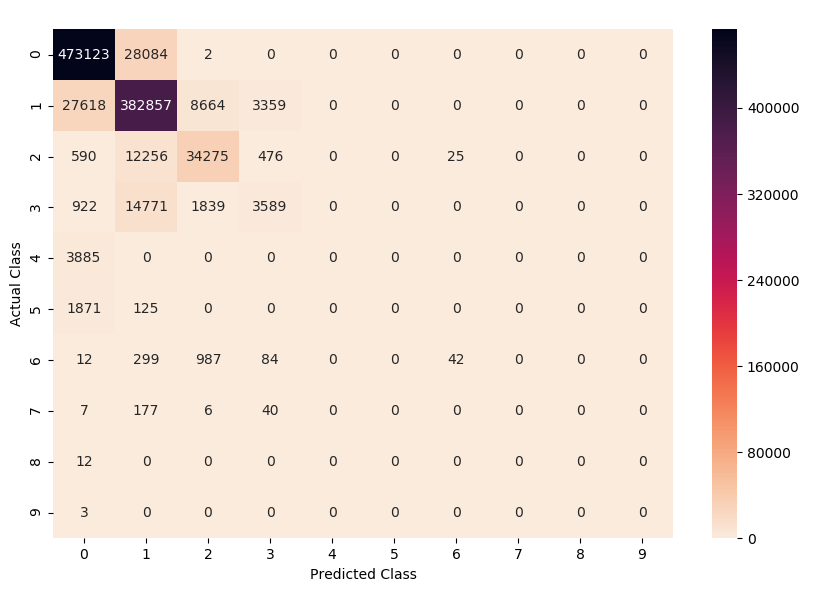
\includegraphics[width=7cm]{chart/d_15.png} }}%
    \subfloat[]{{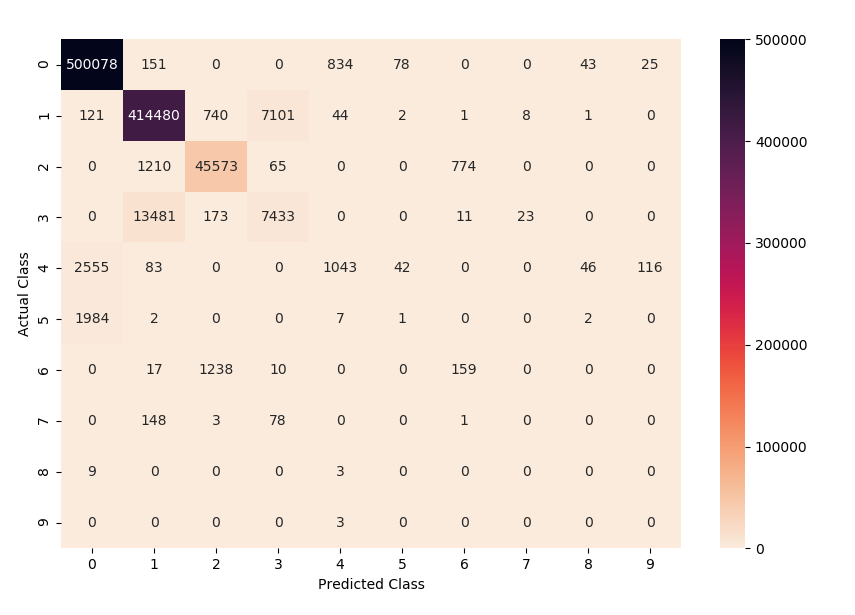
\includegraphics[width=7cm]{chart/d_20.png} }}%
    \subfloat[]{{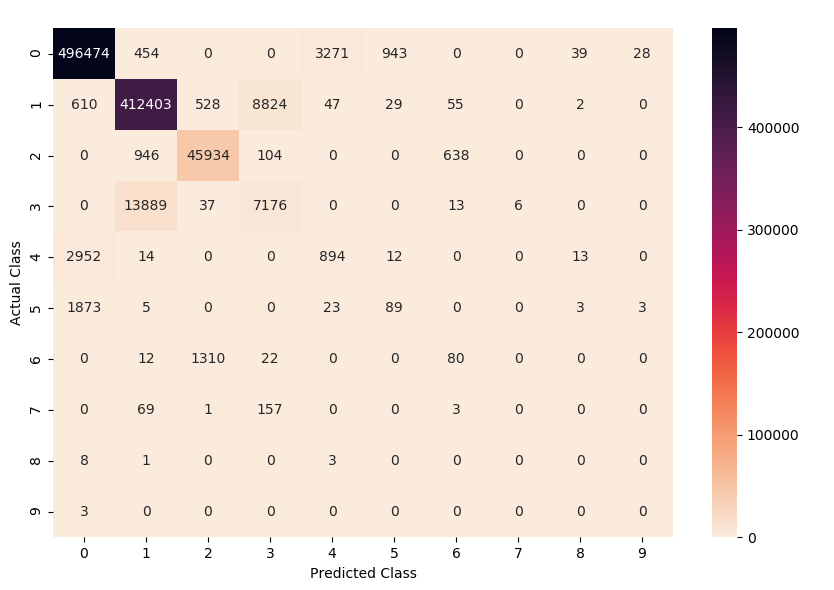
\includegraphics[width=7cm]{chart/d_25.png} }}%
    \caption{Confusion Matrices for hidden layers units = [5,10,15,20,25] for both layers}%
    \label{fig:example}%
\end{figure}
\end{itemize}

% ----------------------


\subsection*{Part (e):}
\begin{itemize}
\item \textbf{Accuracy and Trainig Time:}

\hskip1.0cm\begin{tabular}{ |p{2.7cm}||p{2.5cm}|p{3.3cm}|p{3.3cm}|}
	 \hline
	 % \multicolumn{3}{|c|}{Training Time(in Sec)} \\
	 \hline \textbf{Hiddern Layer Units} & \textbf{Training Time} & \textbf{Training Accuracy} & \textbf{Testing Accuracy}\\
	 \hline
	 5 &  6.09 sec & 54.10\% &  54.17\% \\
	 10 & 8.7 sec & 73.02\% &  71.56\% \\
	 15 & 24 sec & 79.47\% &  77.62\% \\
	 20 & 31 sec & 95.44\% &  94.5\% \\
	 25 & 20.14 sec & 95.04\% &  93.53\% \\
	 \hline
\end{tabular}


\begin{figure}[H]
\centering
	\begin{floatrow}
	\hspace*{-0.9in}
	  \ffigbox[\FBwidth]{\caption{\small{Training time vs No. of Hidden Layer Units}}}{%
	  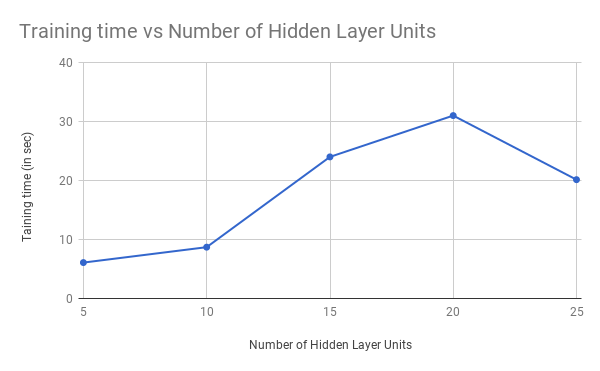
\includegraphics[width=100mm]{chart/es_time.png}
	  }
	  \ffigbox[\FBwidth]{\caption{\small{Training \& Testing Accuracy vs No. of Hidden Layer Units}}}{%
		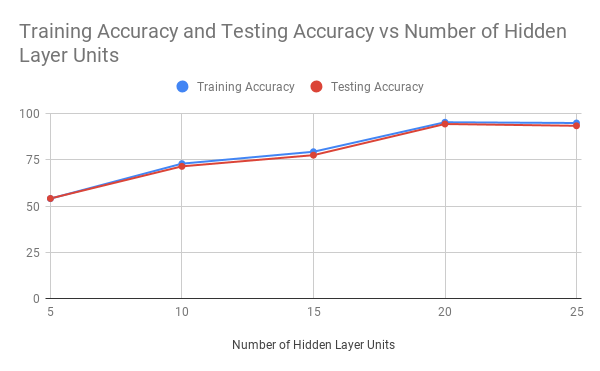
\includegraphics[width=100mm]{chart/es_acc.png}
	  }
\end{floatrow}
\end{figure}


\item \textbf{Confusion Matrices:}
\begin{figure}[H]
    \centering
    \subfloat[]{{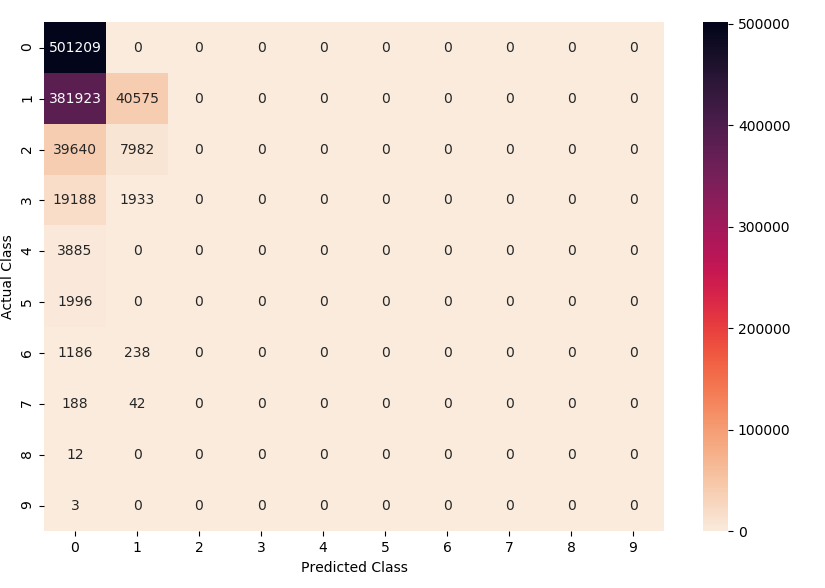
\includegraphics[width=7cm]{chart/e_s5.png}} }%
    \subfloat[]{{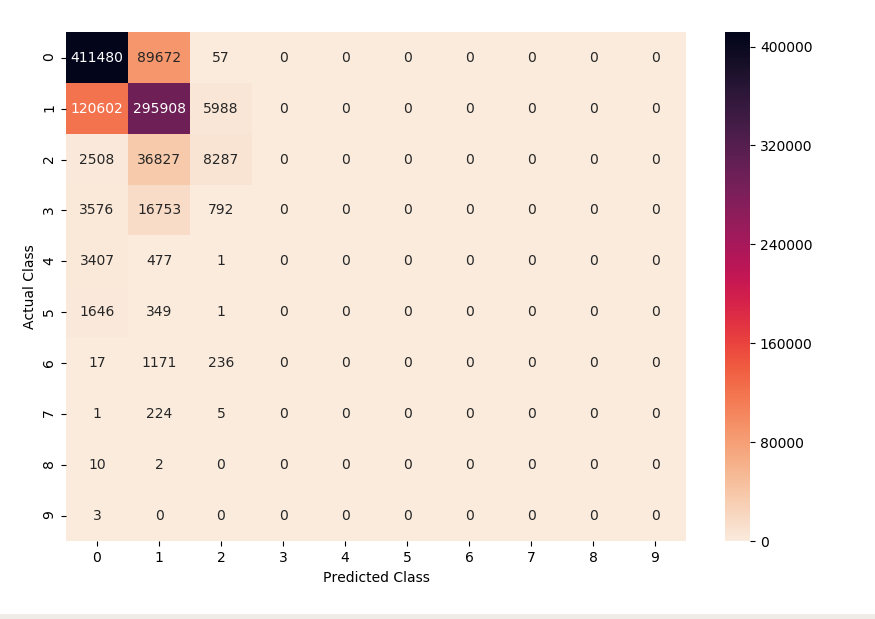
\includegraphics[width=7cm]{chart/e_s10.png} }}%
    \qquad
  	\hspace*{-1.5cm}
    \subfloat[]{{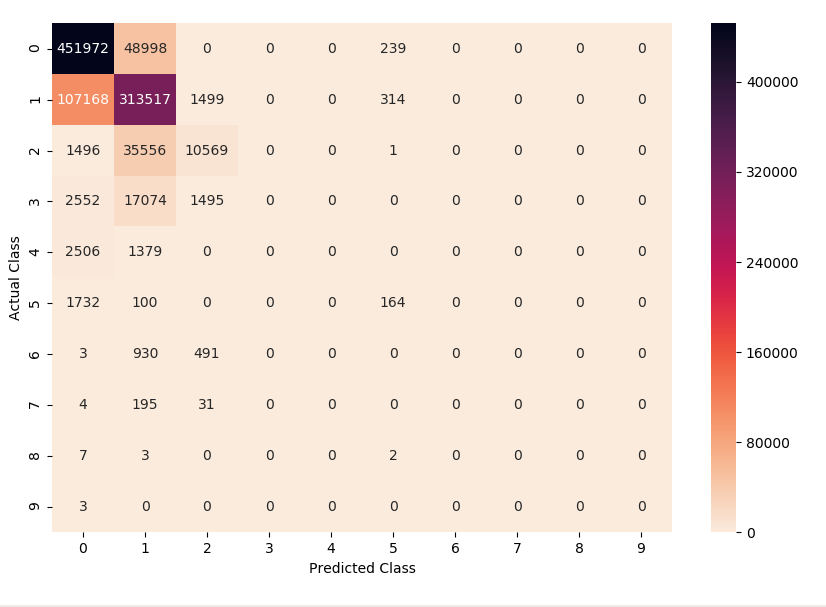
\includegraphics[width=7cm]{chart/e_s15.png} }}%
    \subfloat[]{{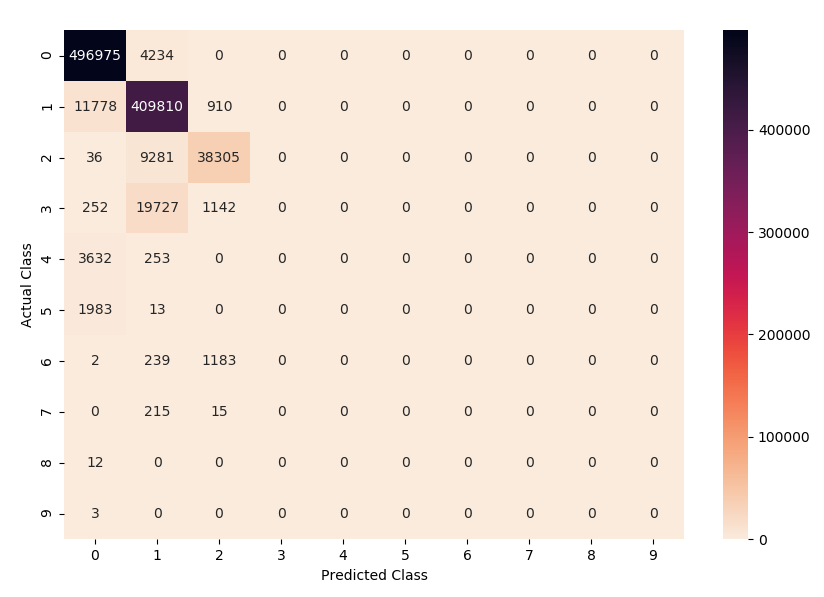
\includegraphics[width=7cm]{chart/e_s20.png} }}%
    \subfloat[]{{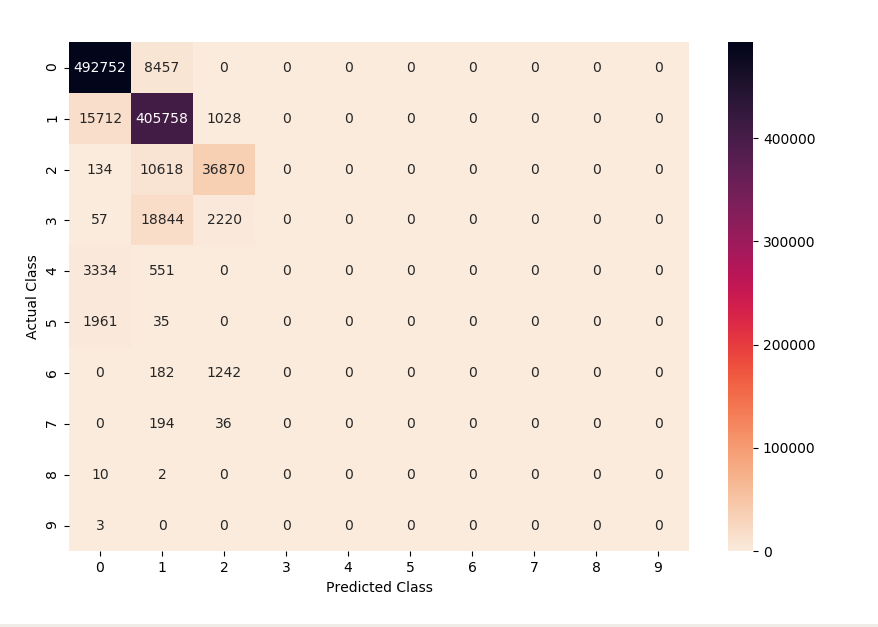
\includegraphics[width=7cm]{chart/e_s25.png} }}%
    \caption{Confusion Matrices for hidden layers units = [5,10,15,20,25]}%
    \label{fig:example}%
\end{figure}
\end{itemize}

% ----------------------

\subsection*{Part (f): ReLU}
\begin{itemize}
\item \textbf{Accuracy and Trainig Time:}

\hskip1.0cm\begin{tabular}{ |p{2.7cm}||p{2.5cm}|p{3.3cm}|p{3.3cm}|}
	 \hline
	 % \multicolumn{3}{|c|}{Training Time(in Sec)} \\
	 \hline \textbf{Hiddern Layer Units(for both layers)} & \textbf{Training Time} & \textbf{Training Accuracy} & \textbf{Testing Accuracy}\\
	 \hline
	 5 &  158 sec & 57.14\% &  55.70\% \\
	 10 & 194 sec & 79.69\% &  78.56\% \\
	 15 & 239 sec & 90.62\% &  89.38\% \\
	 20 & 294 sec & 98.37\% &  96.87\% \\
	 25 & 397 sec & 99.26\% &  96.30\% \\
	 \hline
\end{tabular}

\begin{figure}[H]
\centering
	\begin{floatrow}
	\hspace*{-0.9in}
	  \ffigbox[\FBwidth]{\caption{\small{Training time vs No. of Hidden Layer Units}}}{%
	  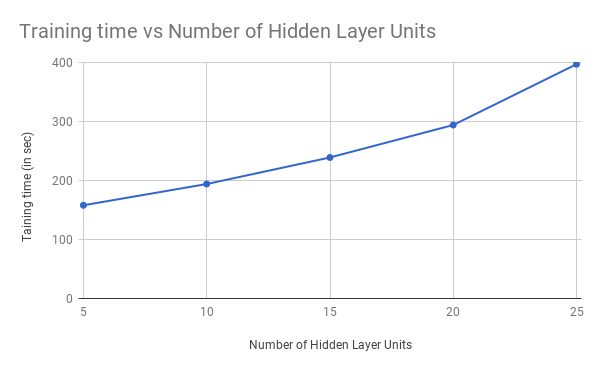
\includegraphics[width=100mm]{chart/d_time.png}
	  }
	  \ffigbox[\FBwidth]{\caption{\small{Training \& Testing Accuracy vs No. of Hidden Layer Units}}}{%
		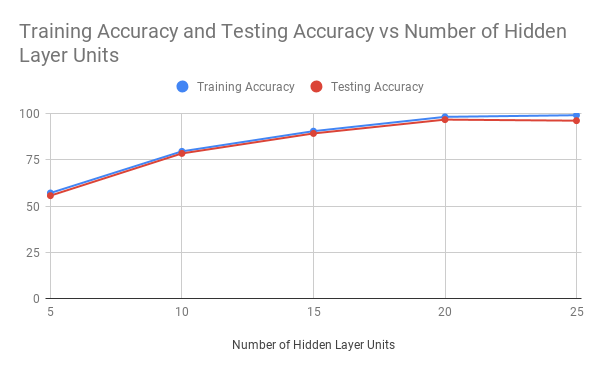
\includegraphics[width=100mm]{chart/d_acc.png}
	  }
\end{floatrow}
\end{figure}


\item \textbf{Confusion Matrices:}
\begin{figure}[H]
    \centering
    \subfloat[]{{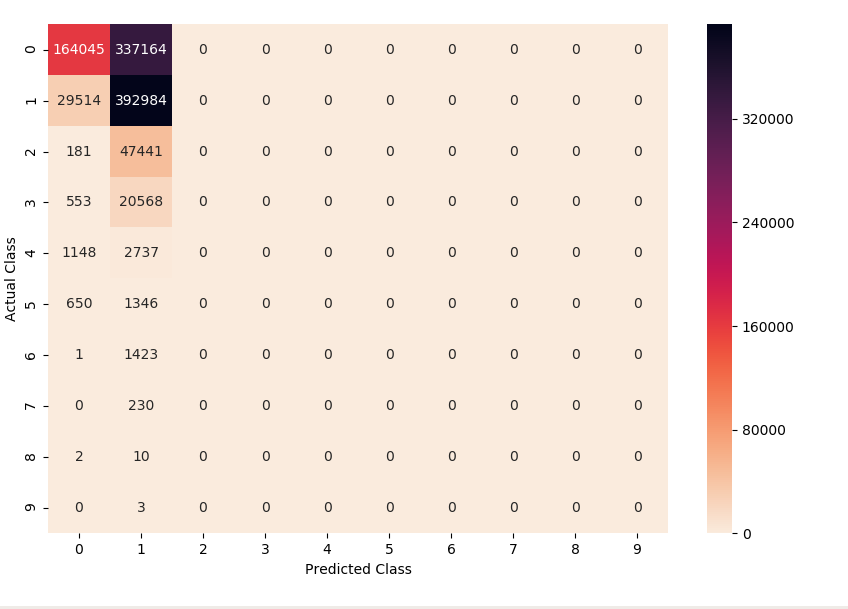
\includegraphics[width=7cm]{chart/d_5.png}} }%
    \subfloat[]{{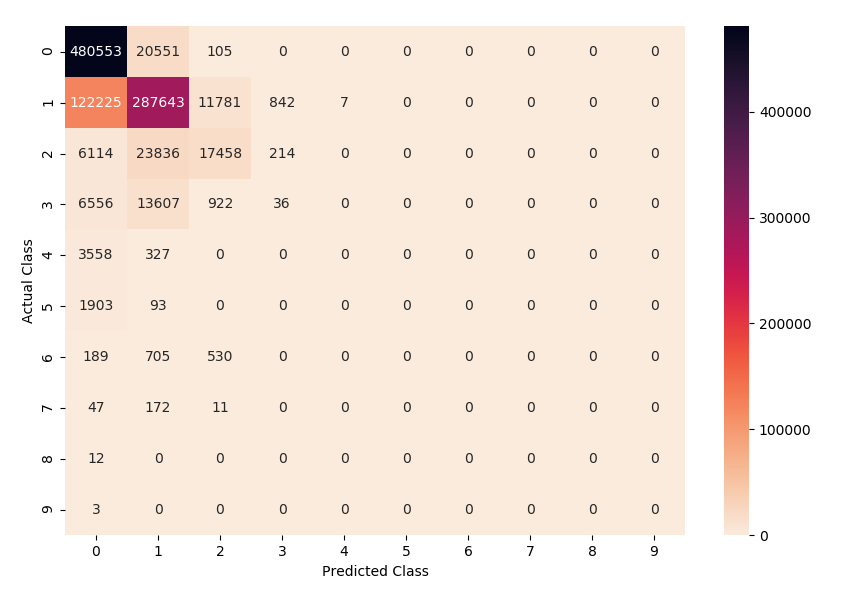
\includegraphics[width=7cm]{chart/d_10.png} }}%
    \qquad
  	\hspace*{-1.5cm}
    \subfloat[]{{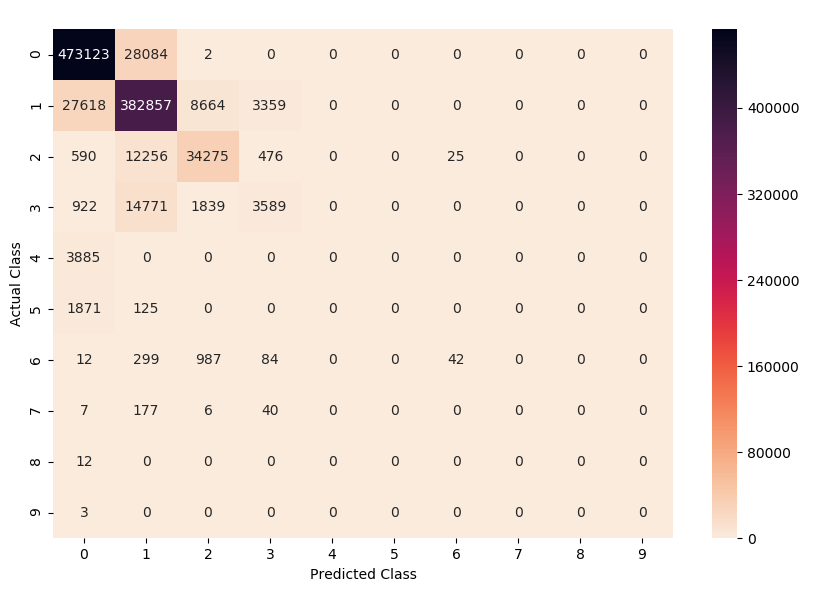
\includegraphics[width=7cm]{chart/d_15.png} }}%
    \subfloat[]{{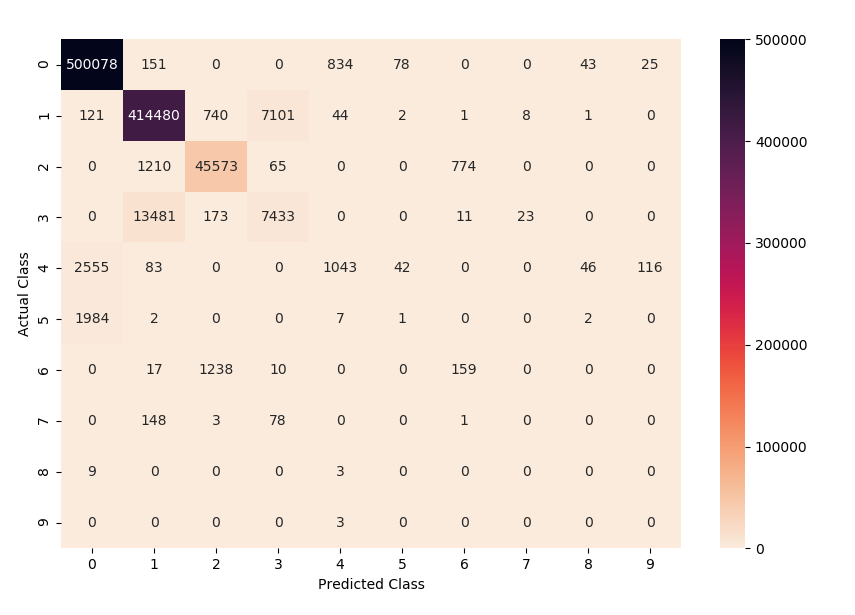
\includegraphics[width=7cm]{chart/d_20.png} }}%
    \subfloat[]{{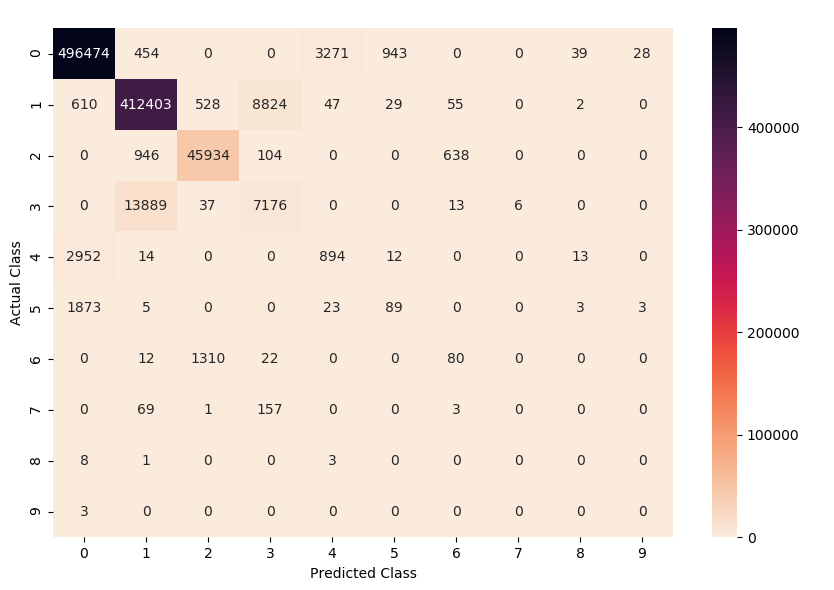
\includegraphics[width=7cm]{chart/d_25.png} }}%
    \caption{Confusion Matrices for hidden layers units = [5,10,15,20,25] for both layers}%
    \label{fig:example}%
\end{figure}
\end{itemize}

% https://drive.google.com/drive/folders/1VVqfcNAuw_i5A9KtQhZJur_dFKMND5h1?usp=sharing
\end{document} 


